\documentclass{amsart}

\usepackage{amsmath,amssymb,graphicx,mathtools,pdfsync,algorithm,algpseudocode,float,hyperref}

\graphicspath{ {../Figures/} }
\begin{document}
	
\title{Monte Carlo Solution to Laplace's Eq on a Rectangular Domain}

\author{Matt Cassini}
\address{Department of Mathematical Sciences, New Jersey Institute of Technology, University Heights, Newark, NJ 07102}
\email{mc225@njit.edu}

\author{Marissah McNeil}
\address{Department of Mathematical Sciences, New Jersey Institute of Technology, University Heights, Newark, NJ 07102}
\email{mm2458@njit.edu}

\author{Moises Ramos}
\address{Department of Mathematical Sciences, New Jersey Institute of Technology, University Heights, Newark, NJ 07102}
\email{mlr4@njit.edu}

\thanks{Math 450H Final Project}
\begin{abstract}
	We use the Tour Du Wino Method, an algorithm based on Monte-Carlo simulation, to approximate a solution to Laplace's Eq on a rectangular domain with Dirichlet boundary conditions
\end{abstract}

\date{\today}
\maketitle



\section{Introduction}
We seek to solve Laplace's Equation

\begin{equation}
	\frac{\partial^2 u}{\partial x^2} + \frac{\partial^2 u}{\partial y^2} = 0
\end{equation}

on a rectangular domain $0 \leq x \leq 7, \quad 0 \leq y \leq 9$ with boundary conditions $u(0,y) = u(7,y) = u(x,0) = 0$ and $u(x,9) = 12$
\section{Background}

In electrostatics the following relationship is known where $E$ represents an electric field, $V$  the electric potential, $\rho$ the charge density and $\epsilon$ the permitivity of the material.

$$E=-\nabla V$$ it is also notable that the electricfield has the following properties physically $$\nabla E= \frac{\rho}{\epsilon}$$ if we do the following to our orginal equation we see an interesting result $$\nabla E=- \nabla \nabla V$$ 
which means $$\nabla ^2 V=- \frac{\rho}{\epsilon}$$ 

If the charge density is zero or in other words if we are in a charge free region or space we arrive at the problem we are interested in LaPlace's Equation
$$\nabla ^2 V=0$$

\section{Implementation}
We programmed a Monte-Carlo simulation using the Tour Du Wino method that utilizes a 2D random walker on a uniform Cartesian grid that records the boundary point on which it lands. It then repeats this process $m$ times starting at this same point. It then averages the value of the boundary condition at each point recorded and assigns this to the value of the solution at the given point.\cite{farlow2012partial}

The proof of this is very straightforward. The expected value for some point a where R(a) is the value it will take is

$ E[R(a)] = \frac{1}{4} (E[R(b)] + E[R(c)] + E[R(d)] + E[R(e)]  )$

where b,c,d, and e are the neighboring points.

This can be rewritten as
\begin{equation}
u_{ij} = \frac{1}{4} (u_{i+1,j} + u_{i-1,j} + u_{i,j+1} + u_{i,j-1})
\end{equation}

which can be rearranged as
\begin{equation*}
u_{i+1,j} + u_{i-1,j} + u_{i,j+1} + u_{i,j-1} - 4u_{ij} = 0
\end{equation*}

The centered finite difference approximations for the second partial derivatives are

\begin{equation*} 
	u_{xx} = \frac{u_{i+1,j} + u_{i-1,j} - 2u_{i,j}}{h^2} \quad u_{yy} = \frac{u_{i,j+1} + u_{i,j-1} - u_{ij}}{h^2}
\end{equation*}

It is now clear the above formulation can be expressed as $h^2 u_{xx} + h^2 u_{yy} = 0$ and dividing away $h^2$ leaves us $u_{xx} + u_{yy} = 0$ which is then Laplace's Eq.

Our initial algorithm was
\begin{algorithm}
	\caption{Original Tour Du Wino}
	\begin{algorithmic}[1]
		\State Initialize $pos1$ and $pos2$ as the first interior coordinate pair
		\State Generate random number $r = \thicksim U(0,1)$
		\If{$r \leq 0.25$}
			\State $pos1 \gets pos1 + 1$
		\ElsIf{$r \leq 0.5$}
			\State $pos1 \gets pos1 - 1$
		\ElsIf{$r \leq 0.75$}
			\State $pos2 \gets pos2 + 1$
		\Else
			\State $pos2 \gets pos2 - 1$
		\EndIf
		\If{$pos1$ or $pos2 == 1$ or $n$}
			\State Save and continue to next starting point
		\Else
			\State Repeat
		\EndIf
		\State Repeat for all starting points
	\end{algorithmic}
\end{algorithm}

This was incredibly slow so we parallelized the algorithm and have the following
\begin{algorithm}
	\caption{Improved Tour Du Wino}
	\begin{algorithmic}[1]
		\State Initalize $pos1$ and $pos2$ as all the coordinate pairs in $2:n-1$, repeated m  times
		\State Create 2 $1 \times n^2m$ arrays, $r$, to store coordinates for each walker
		\State Generate $1 \times n^2m$ array $\thicksim U(0,1)$
		\If{$\quad r_i \leq 0.25$}
			\State $pos1_i \gets pos1_i + 1$
		\ElsIf{$r_i \leq 0.5$}
			\State $pos1_i \gets pos1_i - 1$
		\ElsIf{$r_i \leq 0.75$}
			\State $pos2_i \gets pos2_i + 1$
		\Else
			\State $pos2_i \gets pos2_i - 1$
		\EndIf
		\If{$pos1_i$ or $pos2_i == (1$ or $n)$}
			\State Remove $pos1_i$ and $pos2_i$ from list
			\State Decrease length of random number array
		\EndIf
		\State Repeat until the array is empty
	\end{algorithmic}
\end{algorithm}

This algorithm has improved efficiency as it can take advantage of parallel computing while immediately deleting all "completed" walkers from the arrays so that it doesn't waste time.
\section{Analytical Solution}

If possible, before using a numerical solution to your problem it is best to have an idea of what your solution is supposed to look like. To reiterate the problem

	$$\frac{\partial^2 u}{\partial x^2} + \frac{\partial^2 u}{\partial y^2} = 0$$

on a rectangular domain $0 \leq x \leq 7, \quad 0 \leq y \leq 9$ with boundary conditions $u(0,y) = u(7,y) = u(x,0) = 0$ and $u(x,9) = 12$ 

To solve this analytically, we used separation of variables by hand. When the boundary conditions were applied, the following analytical solution was found
\begin{equation}
    u(x,y)= \sum _{n=1}^{\infty} \frac{48}{n \pi \sinh(9 \sqrt{\lambda})} \sin(x \sqrt{\lambda}) \sinh(y \sqrt{\lambda})
\end{equation}
Where $\lambda=\frac{n^2 \pi ^2}{7^2}$

\subsection{Analytical Solution Plot} 

Here the analytical solution is displayed from several angles 

\begin{figure}[H]
    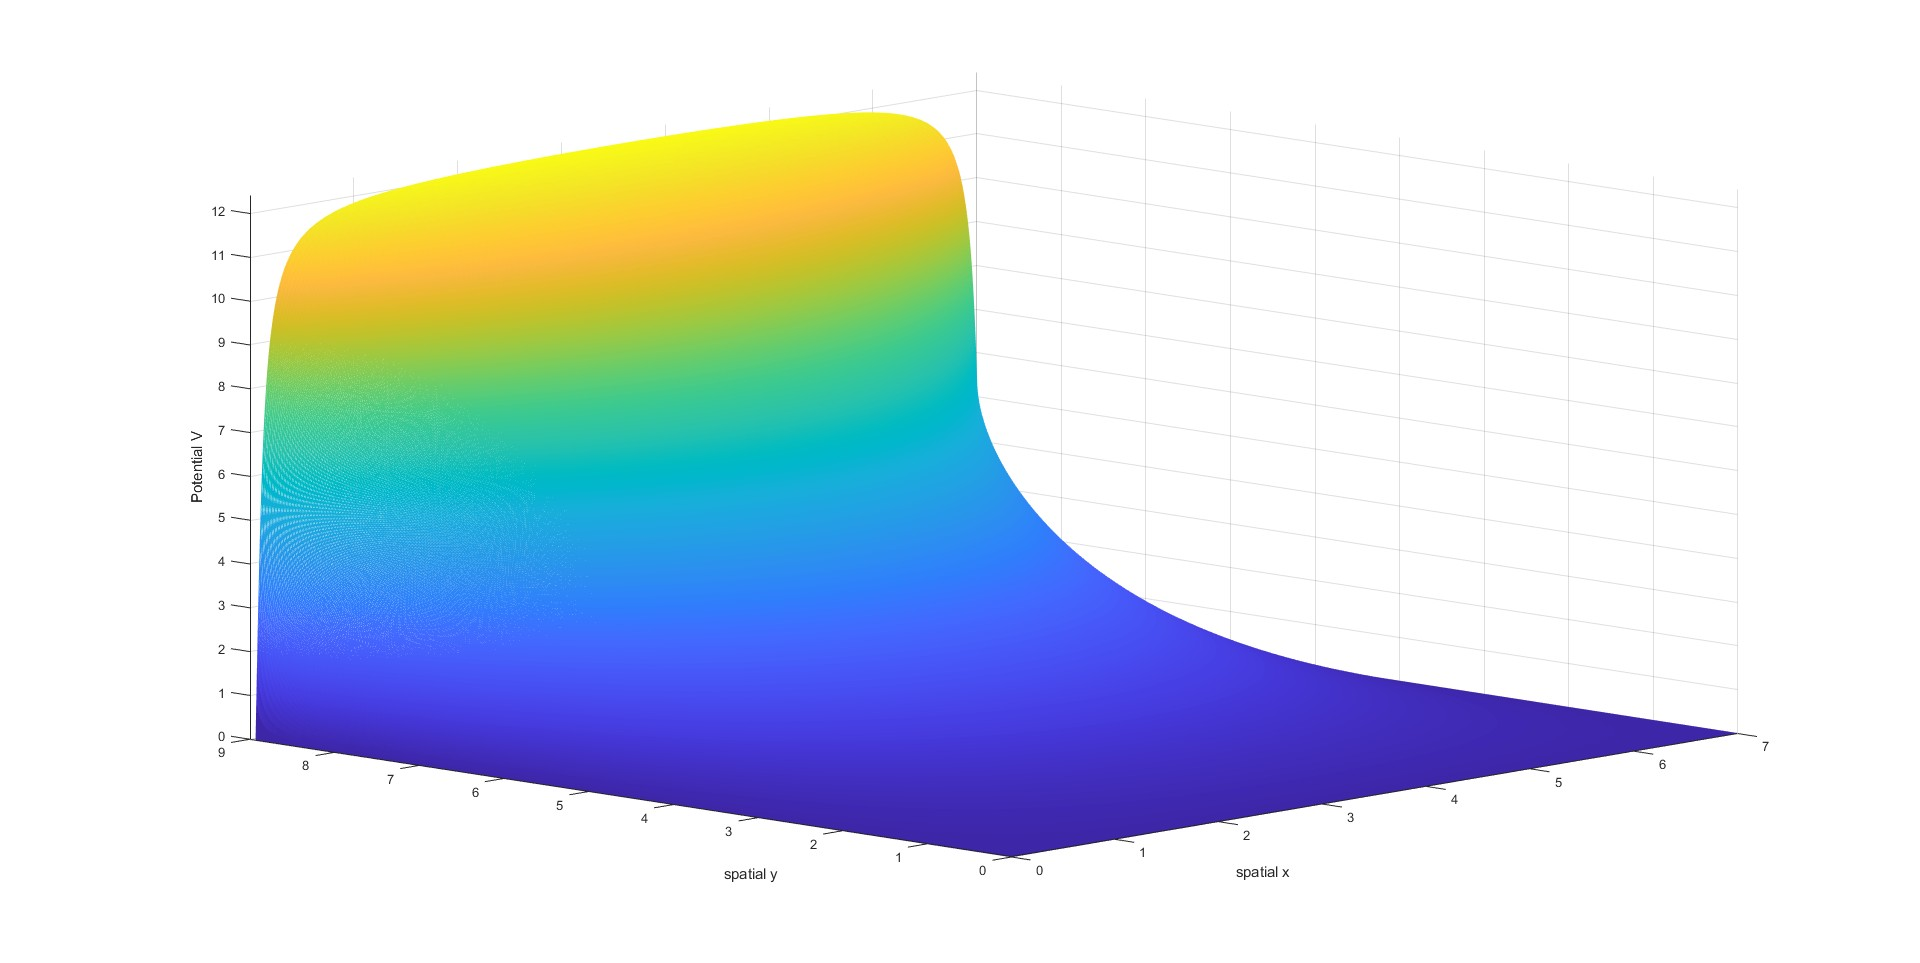
\includegraphics[width=0.6\textwidth]{Asol1.jpg}
\end{figure}
\begin{figure}[H]
    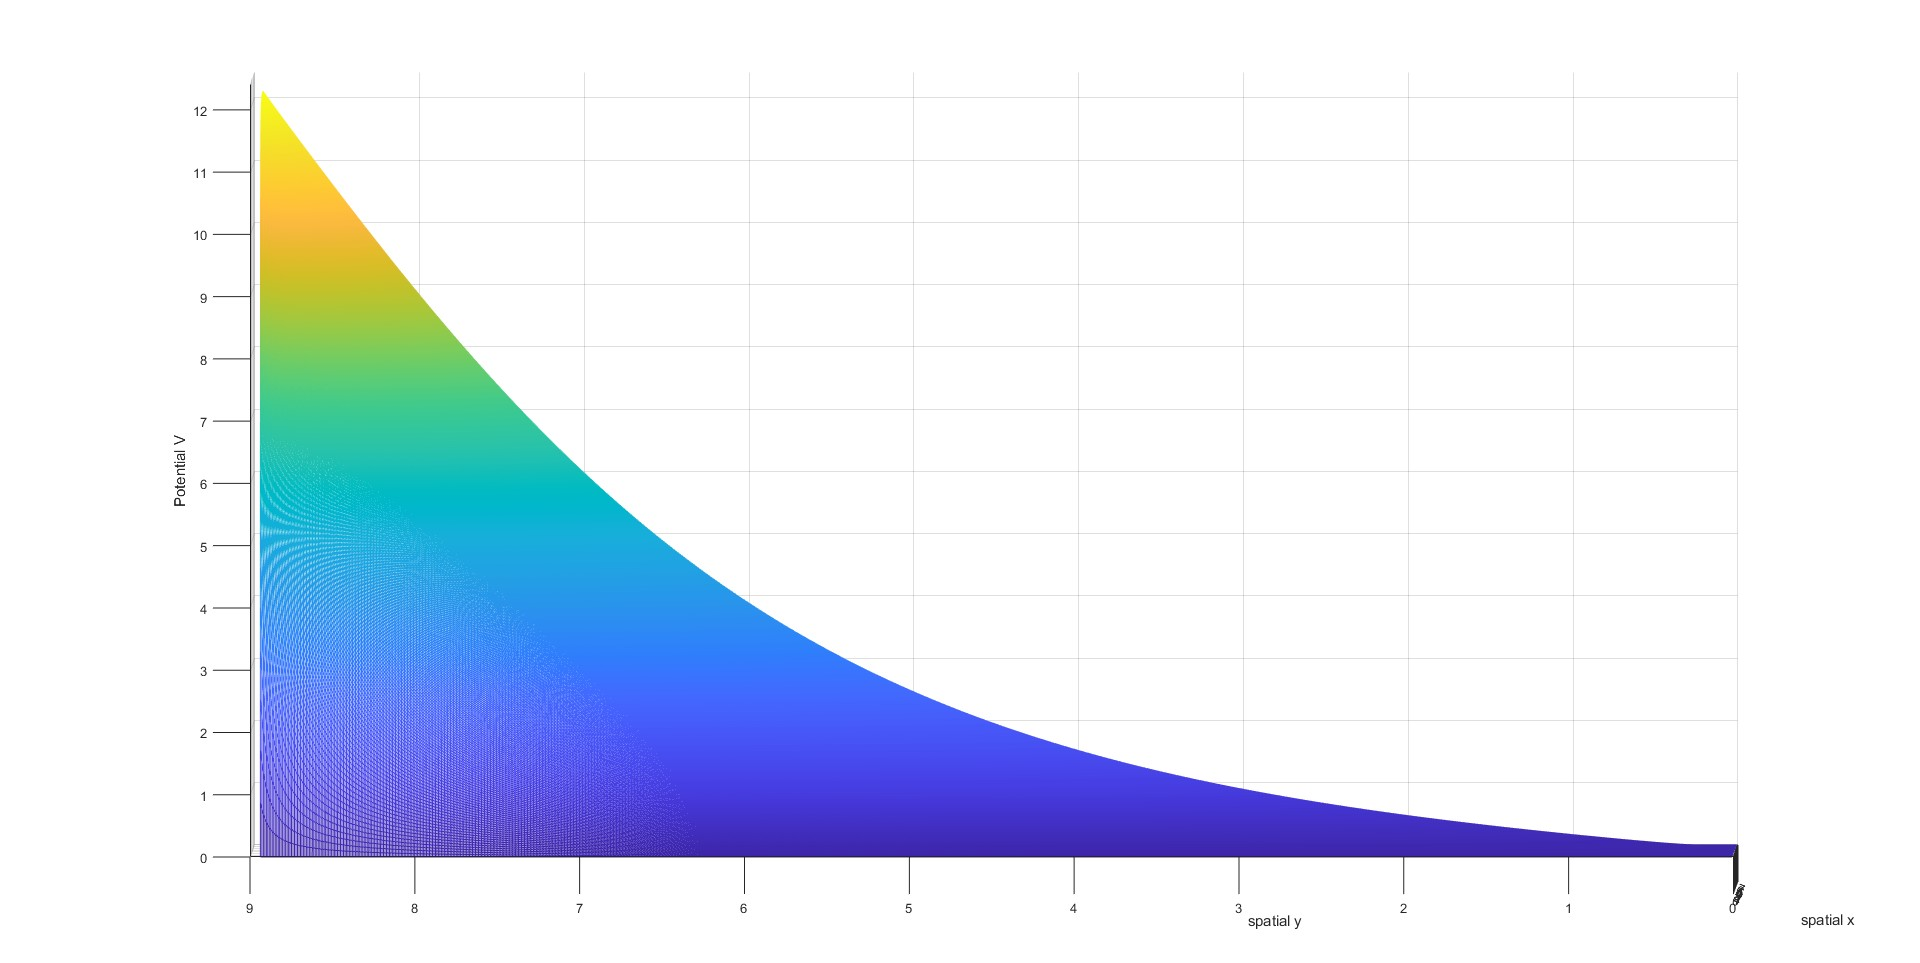
\includegraphics[width=0.6\textwidth]{Asol2.jpg}
\end{figure}
\begin{figure}[H]
    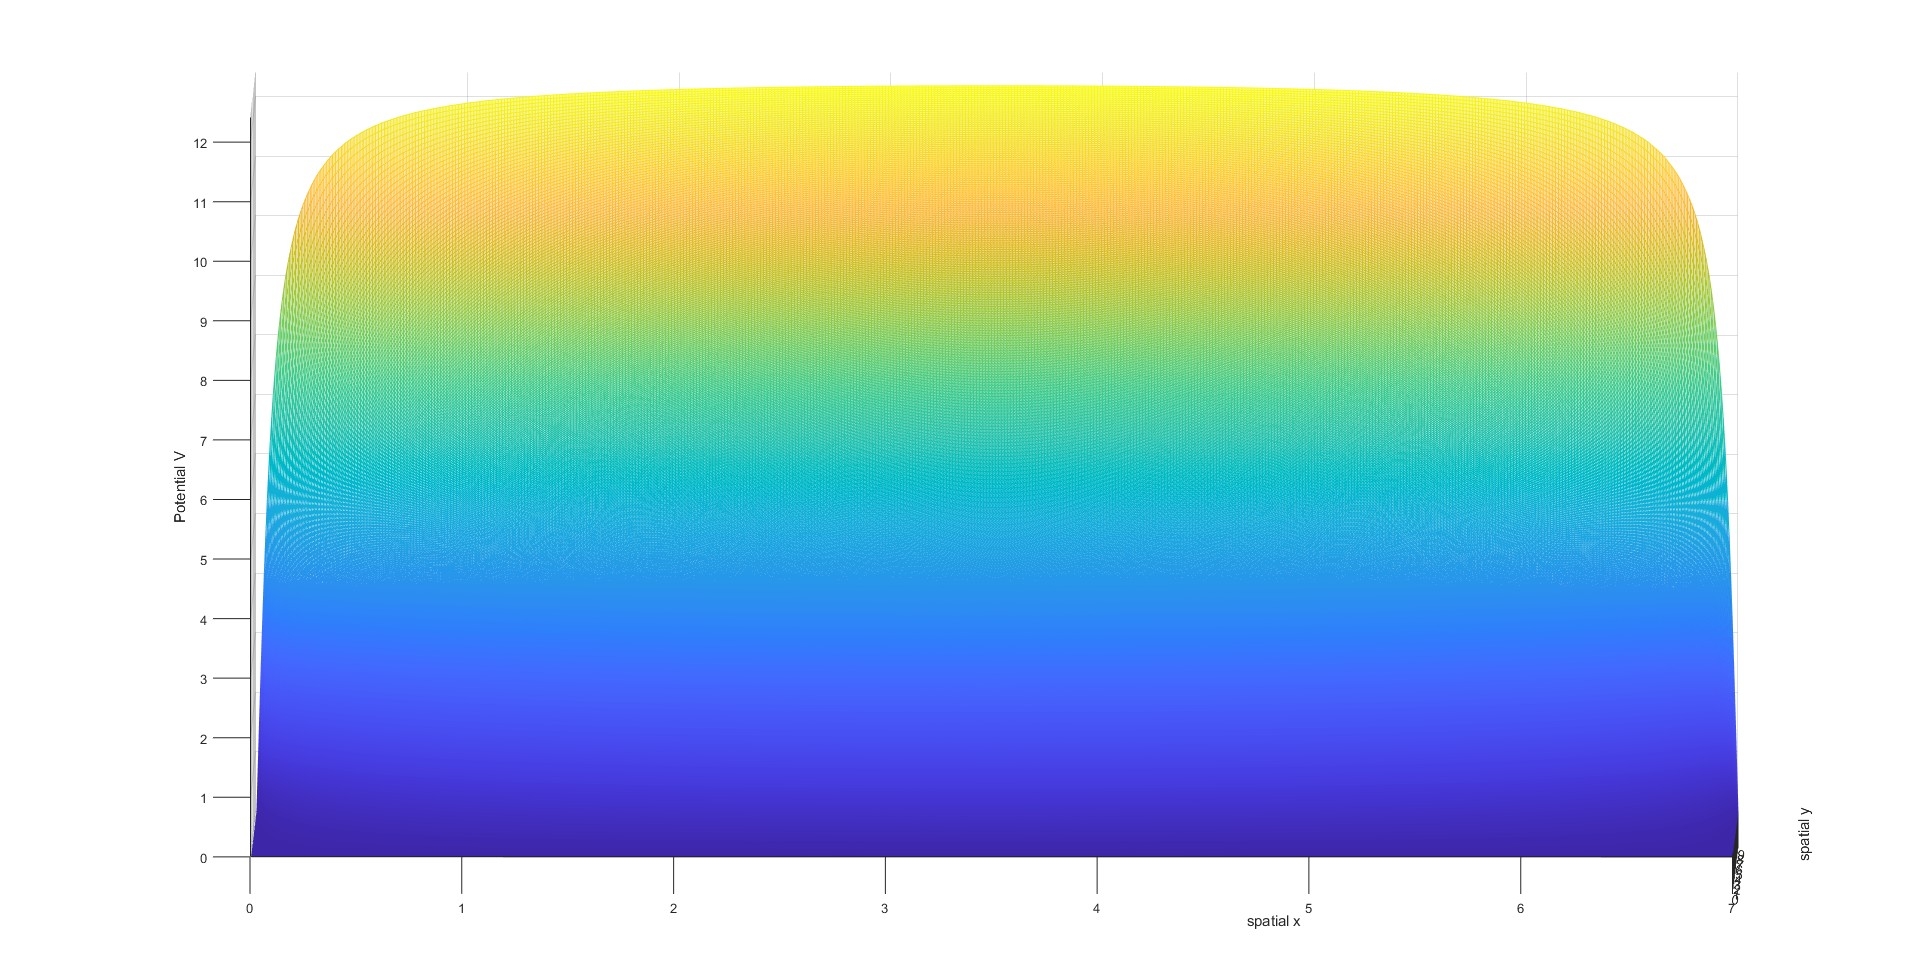
\includegraphics[width=0.6\textwidth]{Asol3.jpg}  
\end{figure}


 \subsection{Analytical Solution Equipotential Lines}
Here we several plots with a different amount of equipotential lines with spatial y as the horizontal axis and spatial x as the vertical axis, which gives an idea of the behavior of the electric potential when it is constant.\\\\
\begin{figure}[H]
    \caption{5 Equipotential Lines}
	\label{5 Equipotential Lines }
	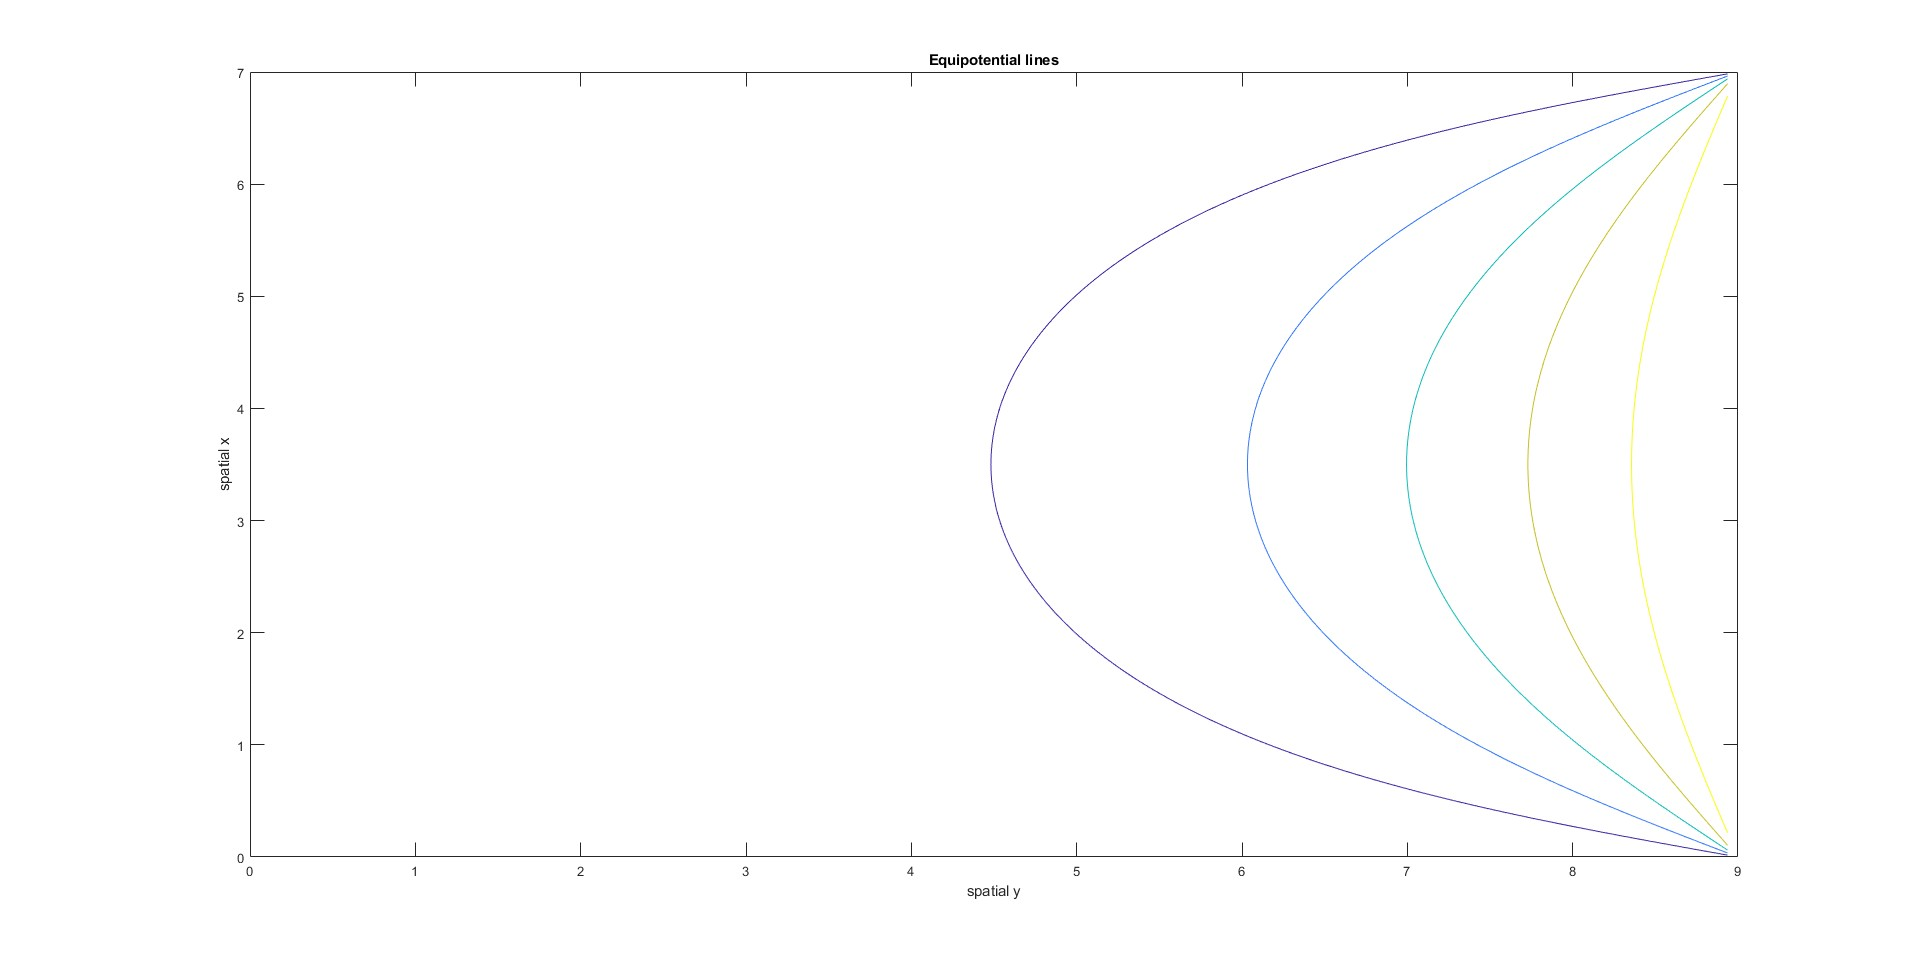
\includegraphics[width=0.48\textwidth]{EL5}
\end{figure}
\begin{figure}[H]
    \caption{15 Equipotential Lines }
	\label{15 Equipotential Lines }
	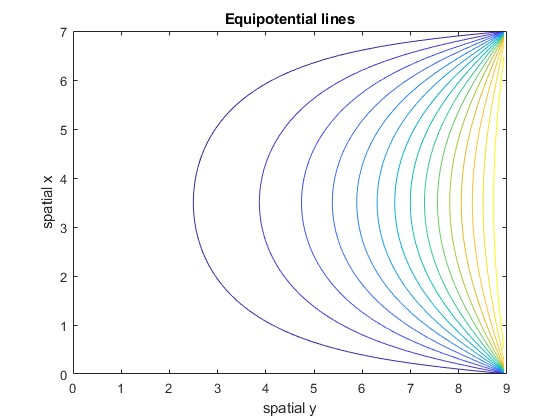
\includegraphics[width=0.48\textwidth]{EL15}
\end{figure}
\begin{figure}[H]
    \caption{20 Equipotential Lines }
	\label{20 Equipotential Lines }
	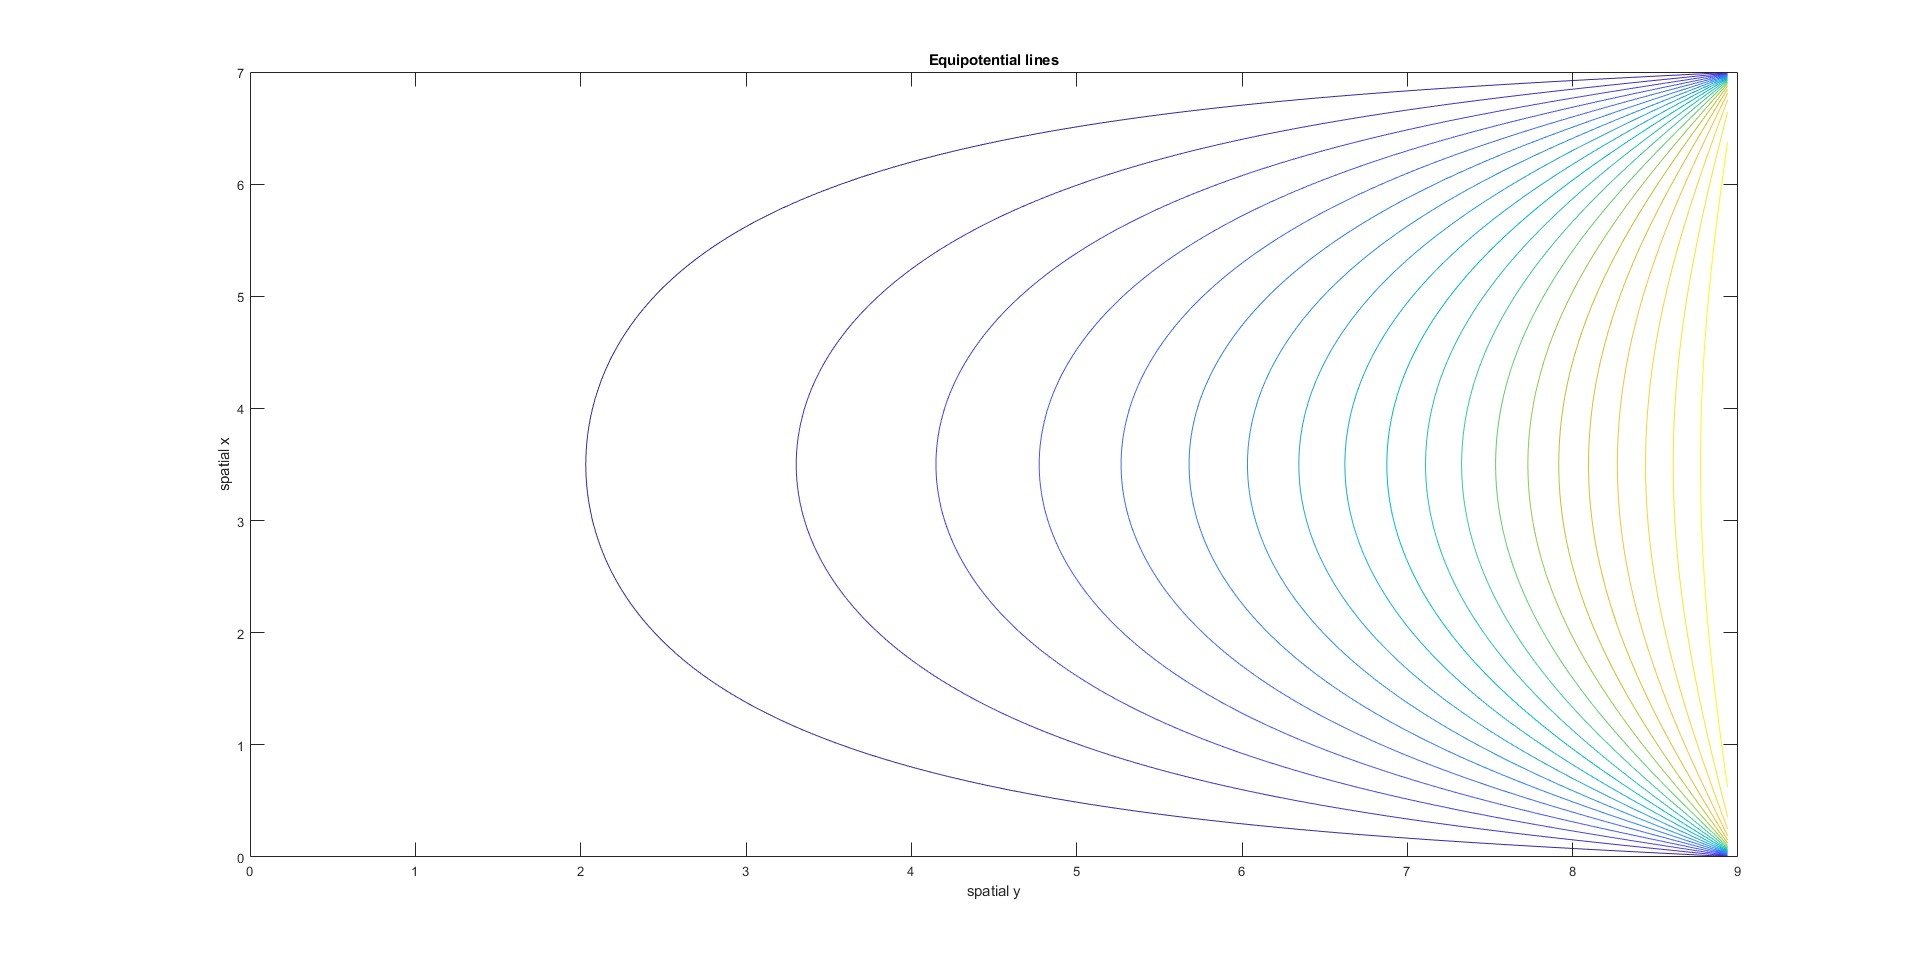
\includegraphics[width=0.48\textwidth]{EL20}
\end{figure}

\section{Computational Results}

\subsection{Plots}

\begin{figure}[H]
	\caption{Numerical solution with a grid size of 350x350 and 350 realizations}
	\label{finalsolution}
	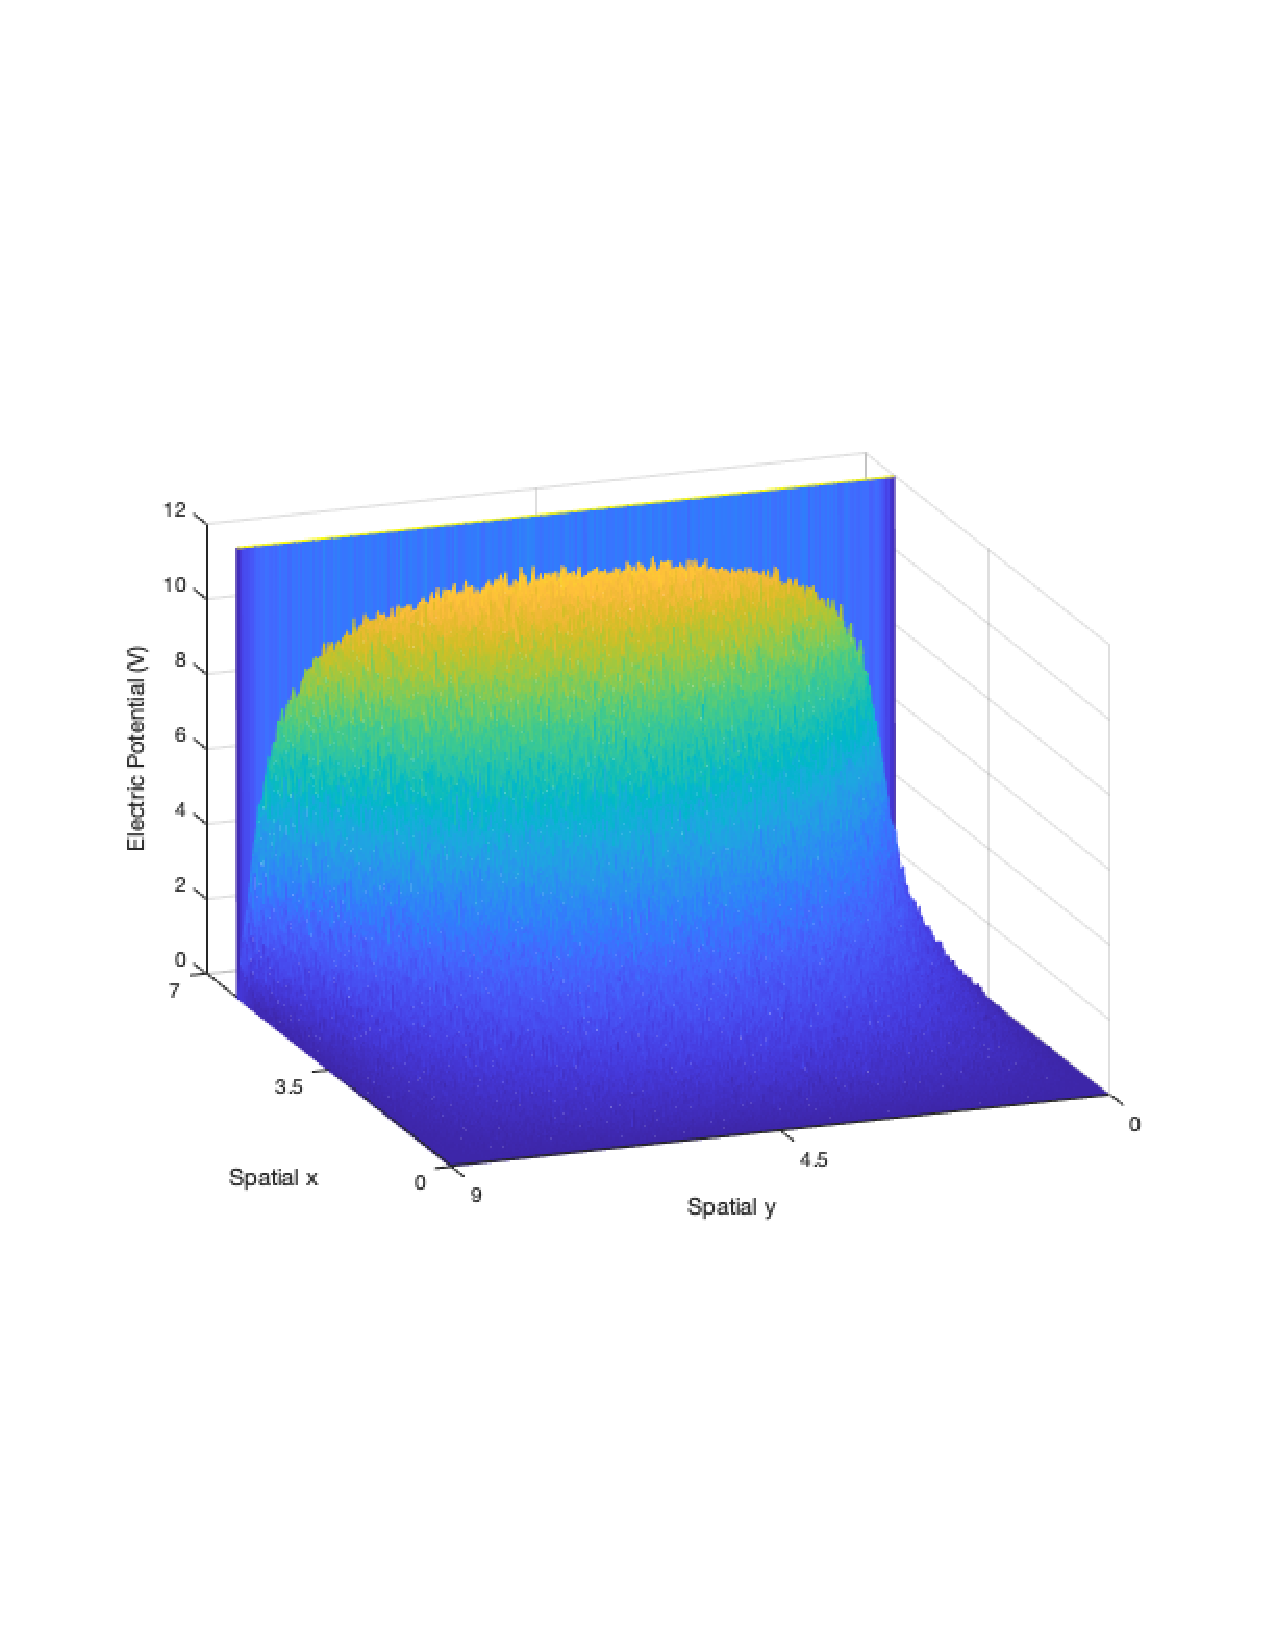
\includegraphics[width=0.48\textwidth]{solution_Dec11_9hrs_isoview.pdf}
	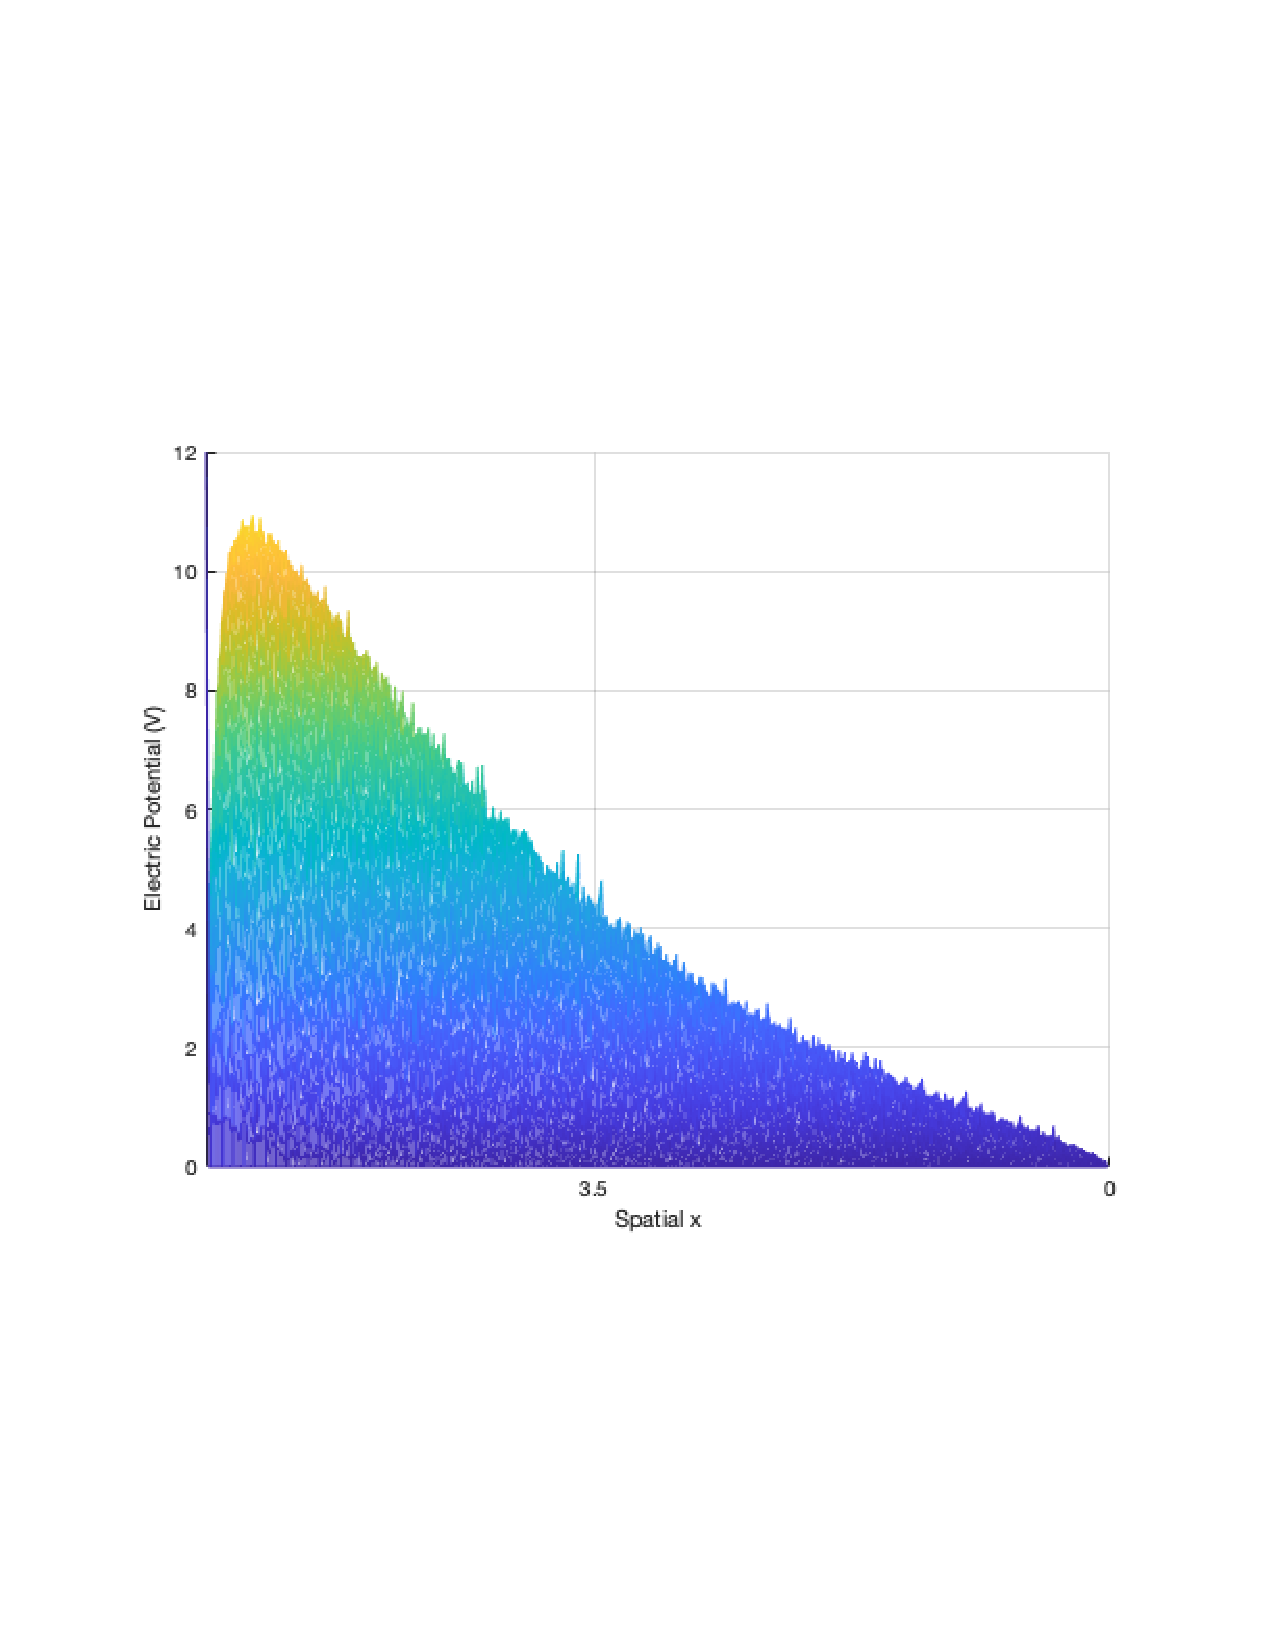
\includegraphics[width=0.48\textwidth]{solution_Dec11_9hrs_sideview.pdf}
\end{figure}

\subsection{Convergence Towards Analytical Solution}

For a small grid size $n$, the solution has significant error regardless of number of trials, $m$.

\begin{figure}[H]
	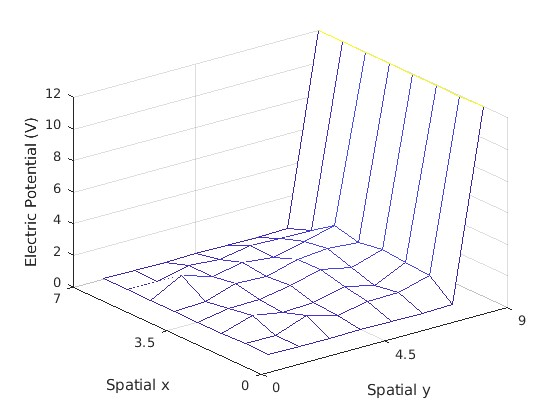
\includegraphics[width=0.48\textwidth]{solution_n=8_m=100.jpg}
	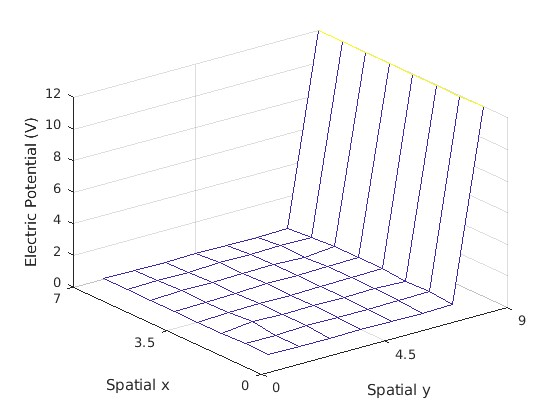
\includegraphics[width=0.48\textwidth]{solution_n=8_m=1000.jpg}
	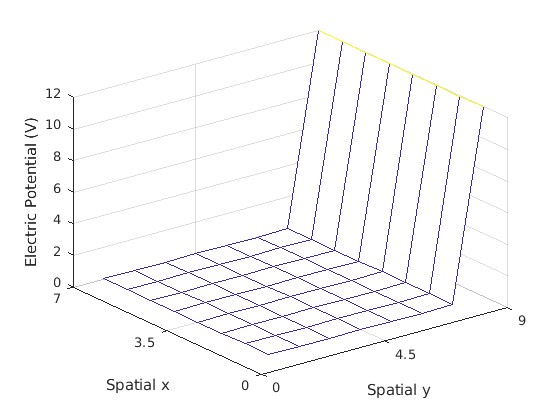
\includegraphics[width=0.48\textwidth]{solution_n=8_m=10000.jpg}
\end{figure}

Clearly, a larger grid size is necessary to see results. By setting $n=m=350$, we obtain Figure \ref{finalsolution} above.

\subsection{Computation Time}

We tested various different grid sizes and number of trials as seen above. We have found the computation time to be $O(n^4m^2)$ where n is the size of the grid and m is the number of trials.

For $n = 8$ and $m = 10,000$, the computation time was 0.47 seconds. For the final solution plot above, we used $n = m = 350$ and found the computation time to be 553 minutes or approximately 9.2 hours.

\section{Discussion}
We have found that the Tour Du Wino is effective in solving Laplace's Equation on a rectangular domain with Dirichlet boundary conditions which allows for a simulation of electric potential from a line charge diffusing through a rectangular domain. An important topic to cover is what occurs at the corners of our solution.Near the corner where the 12 V and 0 V boundary conditions meet, the analytic solution behaves reasonably and smoothly increases from 0 to 12 as y increases.
The numerical solution instantly jumps to 12 along the boundary while immediately next to the boundary it rises similar to the analytic solution.


As far as contribution to the project, Matt Cassini wrote the code to implement the Tour Du Wino algorithm and the error convergence, Moises Ramos derived and plotted the analytical solution and made the random walker animation, and Marissah McNeil wrote the code for the equipotential lines.

\bibliographystyle{plain}
\bibliography{citation}
\end{document}
